\documentclass[crop,tikz]{standalone} 
\usepackage{tikz, amsmath, amssymb, graphicx} 

\DeclareMathAlphabet\mathbfcal{OMS}{cmsy}{b}{n}

\newcommand{\Mt}{\mathbfcal{M}}
\newcommand{\Yt}{\mathbfcal{Y}}
\newcommand{\Ft}{\mathbfcal{F}}

\usetikzlibrary{positioning, shapes.geometric} 

\begin{document} 

\begin{tikzpicture} 


 
\node[inner sep=0pt] at (0, 0) {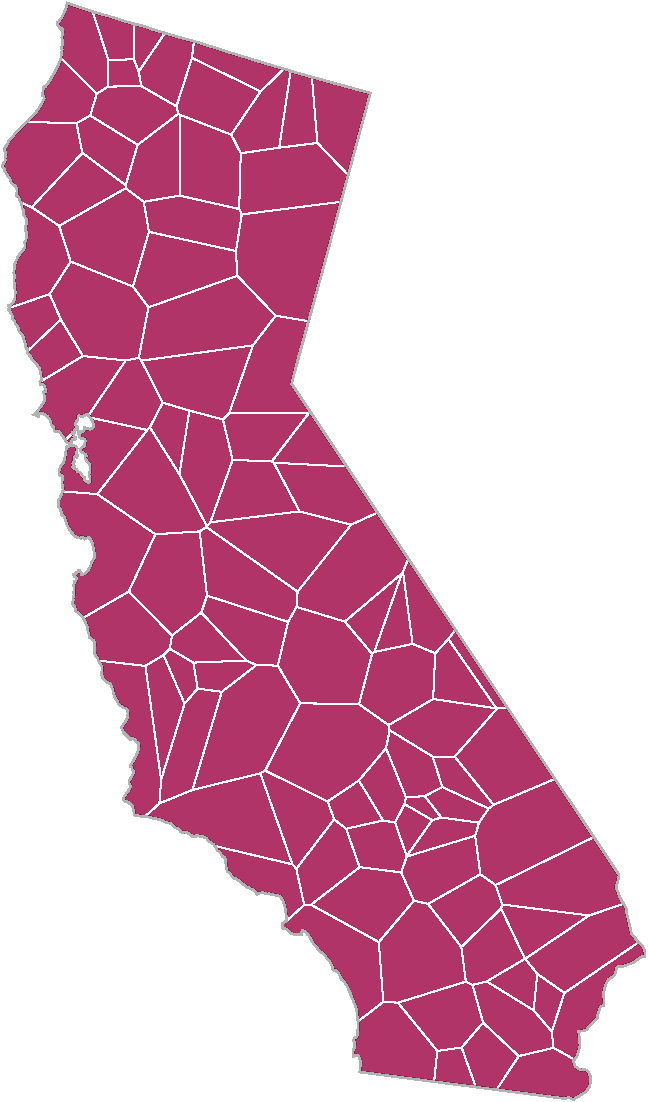
\includegraphics[width=.22\textwidth]{cali_0.pdf}};
\node[inner sep=0pt] at (0, 2.7) {$\lambda_1=0$};


\node[inner sep=0pt] at (3, 0) {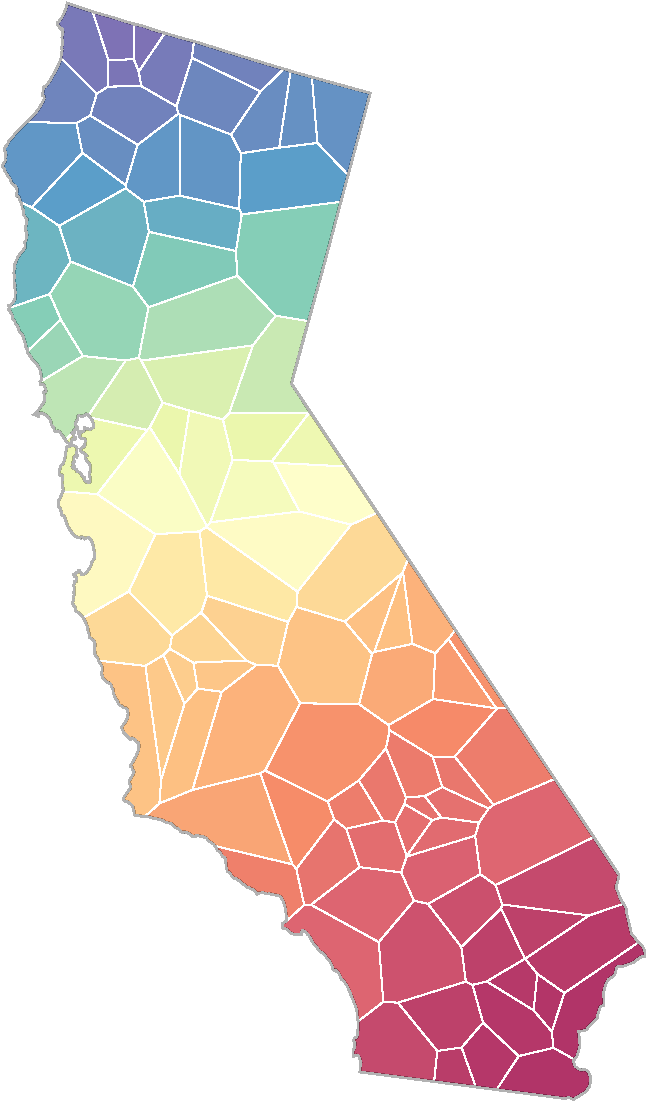
\includegraphics[width=.22\textwidth]{cali_1.pdf}};
\node[inner sep=0pt] at (3, 2.7) {$\lambda_2=0.049$};

\node[inner sep=0pt] at (6, 0) {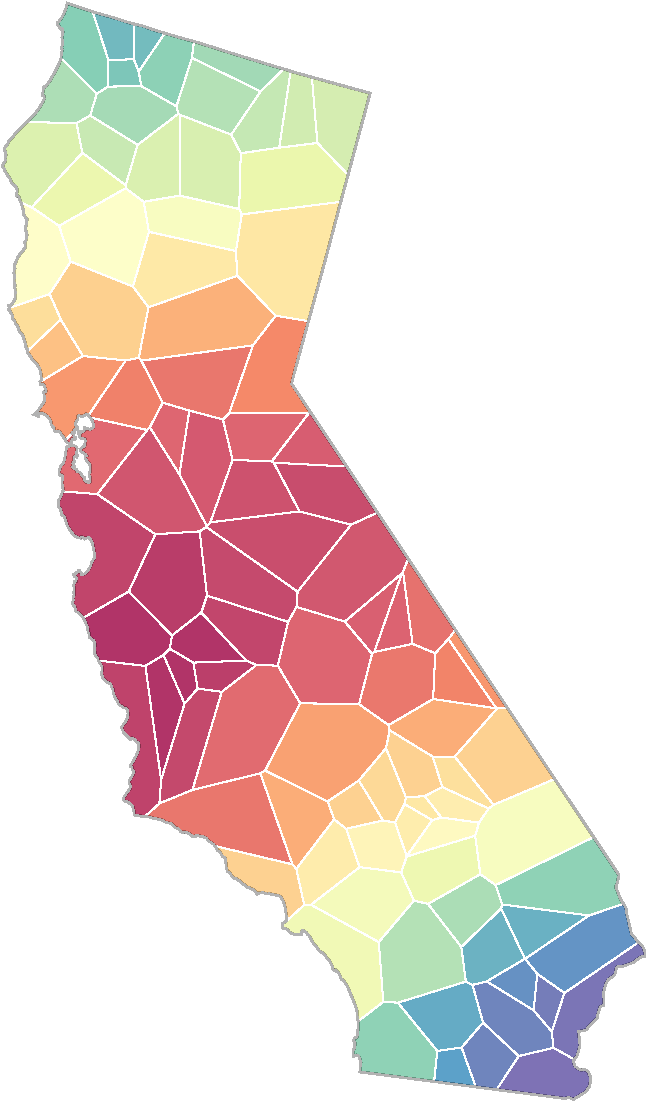
\includegraphics[width=.22\textwidth]{cali_2.pdf}};
\node[inner sep=0pt] at (6, 2.7) {$\lambda_3=0.181$};

\node[inner sep=0pt] at (9, 0) {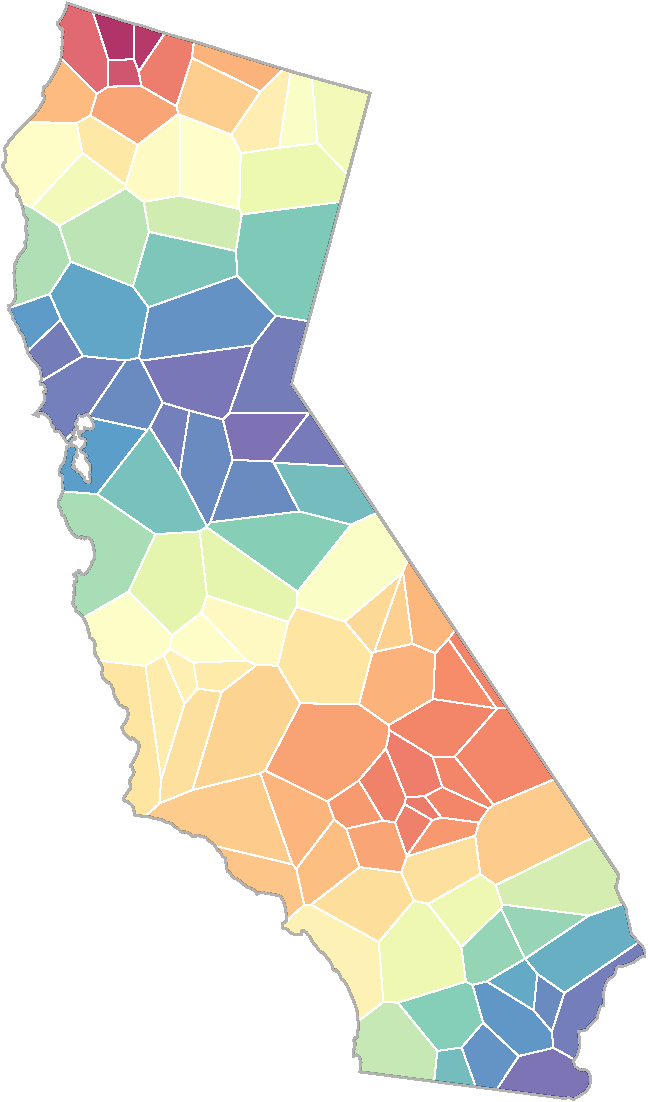
\includegraphics[width=.22\textwidth]{cali_3.pdf}};
\node[inner sep=0pt] at (9, 2.7) {$\lambda_4=0.376$};

\node[inner sep=0pt] at (0, -6) {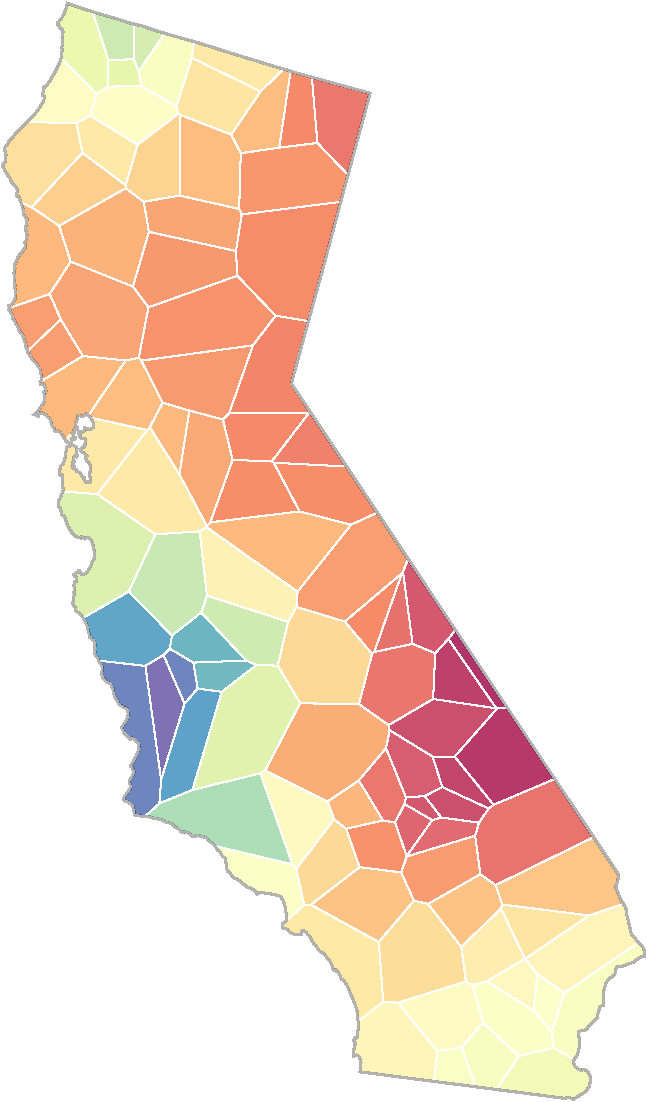
\includegraphics[width=.22\textwidth]{cali_4.pdf}};
\node[inner sep=0pt] at (0, -3.3) {$\lambda_5=0.505$};

\node[inner sep=0pt] at (3, -6) {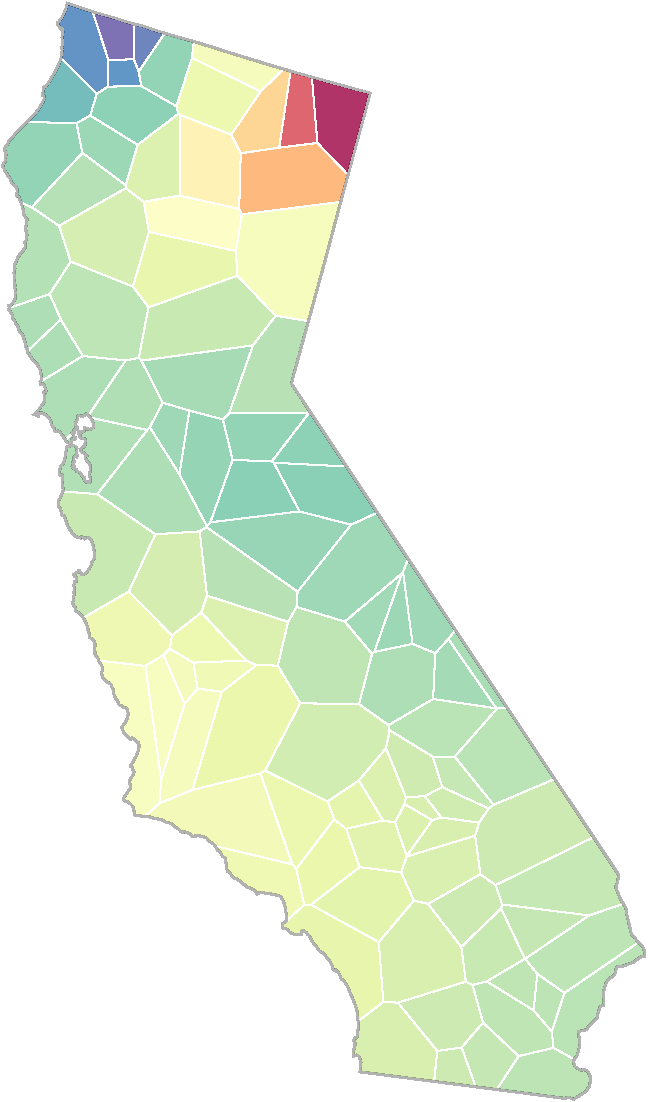
\includegraphics[width=.22\textwidth]{cali_5.pdf}};
\node[inner sep=0pt] at (3, -3.3) {$\lambda_6=0.600$};

\node[inner sep=0pt] at (6, -6) {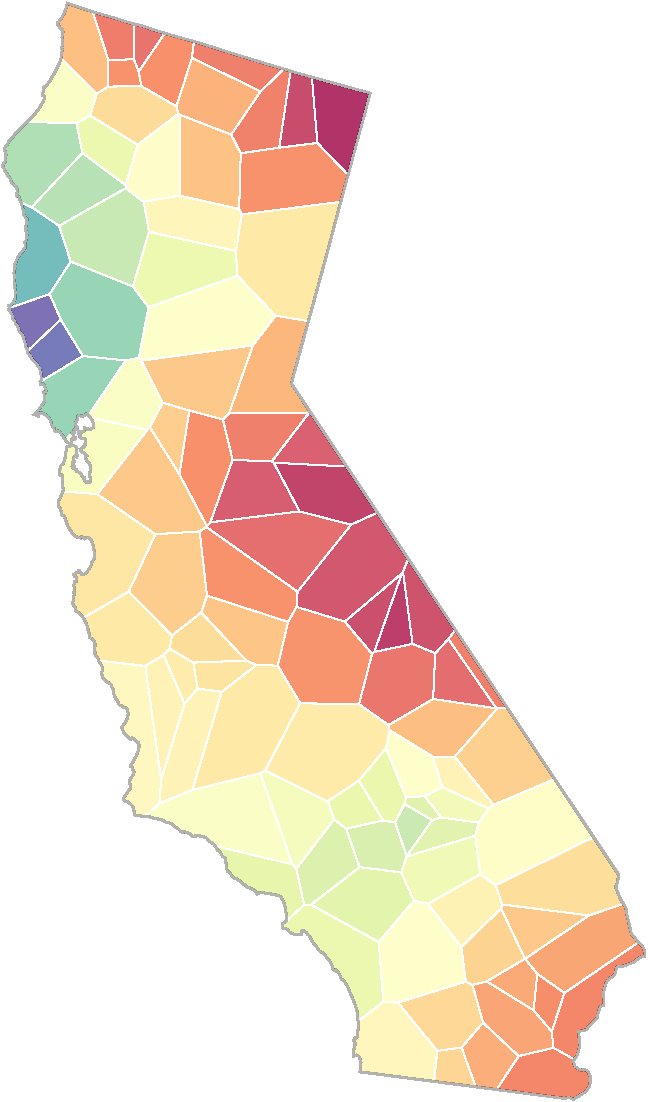
\includegraphics[width=.22\textwidth]{cali_6.pdf}};
\node[inner sep=0pt] at (6, -3.3) {$\lambda_7=0.692$};

\node[inner sep=0pt] at (9, -6) {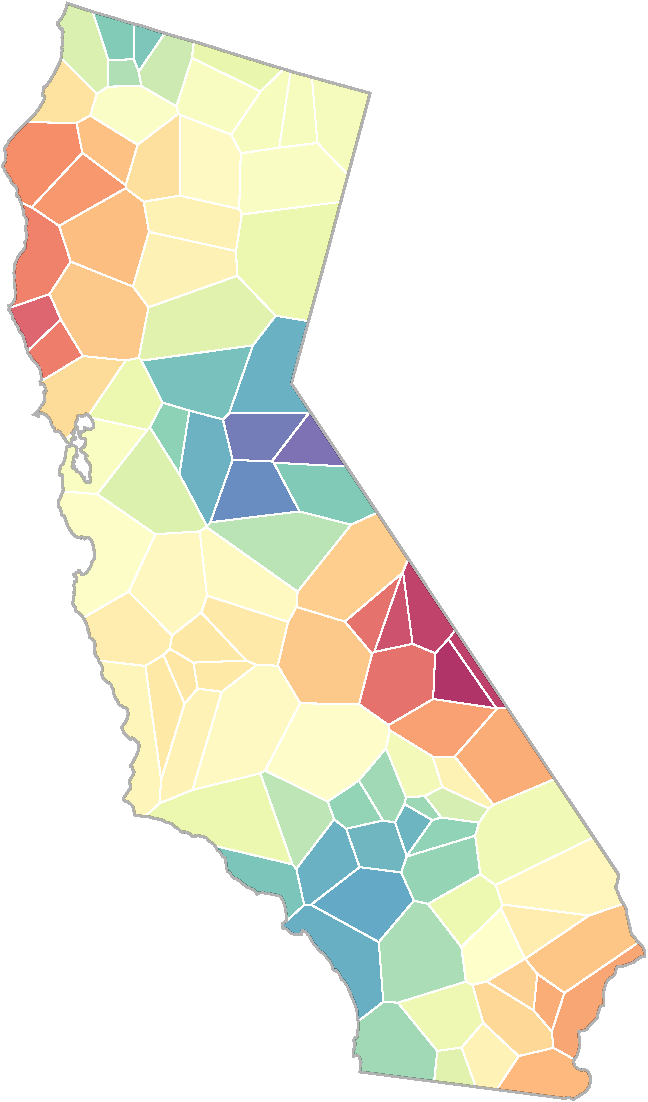
\includegraphics[width=.22\textwidth]{cali_7.pdf}};
\node[inner sep=0pt] at (9, -3.3) {$\lambda_8=0.859$};



 
% \draw [green, dashed] (1, -2.7) rectangle (2.05, 0.3);

% \node [below, opacity=0, text opacity=1] at (2.45, -1) {$\otimes$};

% \draw [blue, dashed] (2.9, -2.7) rectangle (6.5, 0.3);
% \node[inner sep=0pt] (subjects) at (6.2, -0.2) {};

% \node [below, opacity=0, text opacity=1] at (6.9, -1) {$\otimes$};

% \draw [orange, dashed] (7.4, -2.7) rectangle (10.5, 0.3);
% \node[inner sep=0pt] (stimuli) at (10.3, -0.2) {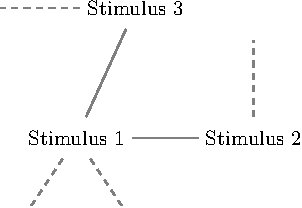
\includegraphics[width=.22\textwidth]{fMRI_Stimuli_Diagram.pdf}};




\end{tikzpicture}
\end{document} 
